\section{Training Framework}
\label{sec:agentic_training_framework}

% \fmh{Why to train open-source LLMs?}
The goal of this section is to train open-source LLMs into reliable ADP agents using reinforcement learning (RL).
However, directly applying RL to this setting is non-trivial due to \textit{sparse reward}, which manifests in two coupled aspects.

(1) {Sparse reward from invalid rollouts.}
Vanilla open-source LLMs are not trained to follow our structured interaction protocol. 
As a result, early in training, the model frequently produces invalid outputs that prevent a meaningful rollout under the agentic tree-based reasoning framework.
Concretely, the model may (1) generate outputs that are not in the action space (e.g., free-form narration, undefined actions, or missing required fields like \texttt{</analyze}), or (2) generate non-executable operators (e.g., invalid operator names, malformed arguments, or Python functions that fail to parse).
Such invalid steps cause immediate termination of environment execution, yielding trajectories that contain little task progress and almost uniformly receive zero reward.
Consequently, RL lacks effective learning signals and struggles to bootstrap.

(2) {Sparse reward from binary task success.}
Even when rollouts are executable, ADP success is typically judged by whether the final generated table matches the target, which induces a binary outcome reward.
This binary supervision ignores \textit{almost-correct} trajectories, for example, a pipeline that correctly performs cleaning and reconstruction for many steps but fails at the end due to a minor schema mismatch or formatting discrepancy.
Assigning the same reward to almost-correct and completely incorrect trajectories severely weakens credit assignment over long horizons, making optimization sample-inefficient.



%!TEX root = ../../main.tex
\begin{figure*}[t]
    \centering 
    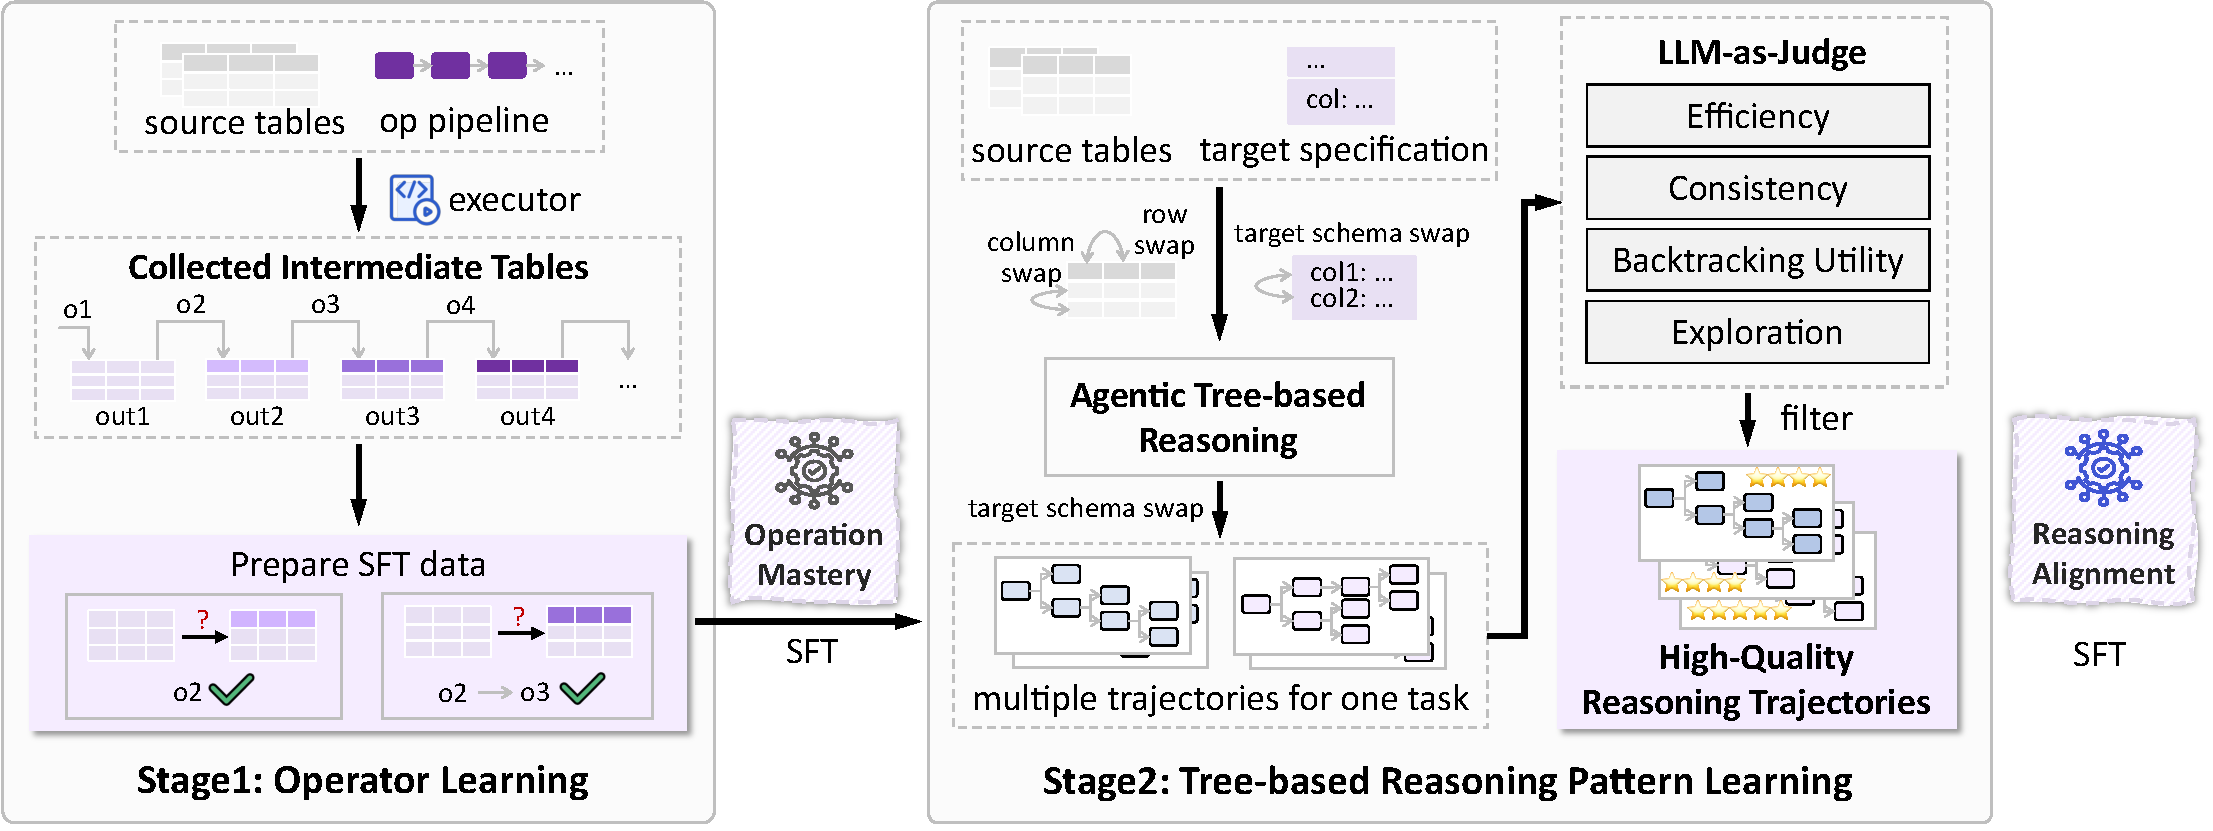
\includegraphics[width=0.9\textwidth]{figures/fig/cold_start.pdf}
  % \vspace{-0.7em}
    \caption{Overview of the progressive cold-start curriculum, which consists of two stages: Operator Learning and Multi-Solution Generation. An LLM-as-Judge mechanism filters these trajectories to ensure high-quality supervision for fine-tuning.
    }
    \label{fig:cold_start}
  % \vspace{-1em}
\end{figure*}

\subsection{Cold-Start}
\label{subsec:cold_start}

Before engaging in reinforcement learning, the agent must acquire a foundational understanding of the operator space and the tree-based reasoning schema. We achieve this via a two-phase supervised alignment strategy.

\stitle{Stage 1: Operator-Level Capability Building.}
The primary objective of this phase is to align the model with the semantics of individual operators (e.g., parameter constraints of \texttt{SplitColumn}) and short-range logical dependencies.
Directly predicting long-horizon pipelines from scratch is challenging for an uninitialized model. To mitigate this, we employ a \textit{sub-sequence modeling} strategy.
Specifically, given a ground-truth pipeline $\Pi_{total}$ (synthesized via the process in Section~\ref{sec:data_synthesis}), we sample continuous sub-sequences $\Pi_{sub} = {o_i, \dots, o_{i+k}}$ (where $k \le 4$).
We execute the prefix of the pipeline to derive the intermediate input table $T_{in}$, and execute $\Pi_{sub}$ to obtain the output table $T_{out}$.
The model is then optimized to reconstruct $\Pi_{sub}$ given the state transition $(T_{in}, T_{out})$:
\begin{equation}
\mathcal{L}_{\text{op}} = -\sum_{(T_{in}, T_{out}, \Pi_{sub}) \in \mathcal{D}_{\text{op}}} \log P_\theta(\Pi_{sub} \mid T_{in}, T_{out})
\end{equation}
This stage effectively functions as a ``vocabulary acquisition'' phase, enabling the model to map table state changes to precise operator calls within a controlled context.

\stitle{Stage 2: Tree-Based Reasoning Pattern Learning.}
Building upon the operator-aware model, this stage aligns the agent with the hierarchical reasoning paradigm of \sys. The goals are twofold: (1) teaching the model to orchestrate the atomic actions (\texttt{<analyze}, \texttt{<expand}, etc.), and (2) ensuring output diversity to broaden the exploration boundary for subsequent RL~\cite{guo2025deepseek}.


As illustrated in Figure~\ref{fig:cold_start} (right), we construct a diverse corpus of reasoning trajectories.
% As illustrated in Figure~\ref{fig:cold_start} (right), we construct a collection of reasoning trajectories as SFT data.
To ensure diversity, for each task $(\mathcal{D}, \mathcal{Q}, T^*)$, we employ $K$ distinct SOTA LLMs (acting as ``teacher'' agents) to generate candidate solution trajectories. We further augment this data via \textit{input perturbation}, randomly permuting row/column orders in $\mathcal{D}$ and schema descriptions in $\mathcal{Q}$. This yields a set of candidate trajectories:
\begin{equation}
\mathcal{S} = \{\tau_k \mid \tau_k \sim f(\tilde{\mathcal{D}}_k, \tilde{\mathcal{Q}}_k, \text{LLM}_k), k = 1, \dots, K\}
\end{equation}

To ensure quality, we employ an \textit{LLM-as-Judge} mechanism to filter out inefficient or redundant reasoning paths. We define a multi-dimensional scoring function:
\begin{equation}
\text{Score}(\tau) = \sum_{d=1}^{4} w_d \cdot f_d(\tau)
\end{equation}
which scrutinizes the trajectory across four dimensions:
(1) {Reasoning Efficiency} (penalizing redundant steps);
(2) {Consistency} (alignment between \texttt{<analyze} thoughts and \texttt{<expand} actions);
(3) {Rollback Utilization} (effectiveness of error correction); and
(4) {Exploration Capability}.
We retain only high-quality trajectories $\mathcal{S}{\text{filtered}}$ where $\text{Score}(\tau) \geq \delta$. The policy is then fine-tuned to maximize the likelihood of these filtered paths:
\begin{equation}
\mathcal{L}{\text{tree}} = -\sum_{\tau \in \mathcal{S}_{\text{filtered}}} \sum{t=1}^{|\tau|} \log P_\theta(a_t \mid \mathcal{T}_t)
\end{equation}
where $a_t$ denotes the action at step $t$ given the state tree $\mathcal{T}_t$.

\subsection{Reward Design}
\label{subsec:rl}

While the cold-start curriculum provides a robust initialization, the model may still struggle with \textit{credit assignment} in unseen, complex scenarios. To optimize the policy for long-horizon robustness, we employ Reinforcement Learning.
A major challenge in DP is the sparsity of the outcome reward ($R_{\text{out}}$). For instance, if a 10-step pipeline fails at the final step due to a minor formatting mismatch, a binary reward of $0$ fails to acknowledge the correctness of the preceding 9 steps, impeding gradient estimation~\cite{lyu2025sql}.

\stitle{Hybrid Reward Design.}
To provide dense, fine-grained supervision, we design a hybrid reward function composed of three synergistic signals:

\noindent (1) \textbf{Partial Reward ($R_{\text{partial}}$).} This component quantifies the structural and semantic proximity between the generated table $\hat{T}$ and the ground truth $T^*$.
\begin{equation}
\begin{cases}
S_{\text{schema}} = \frac{|C_{\hat{T}} \cap C_{T^*}|}{|C_{\hat{T}} \cup C_{T^*}|} \\
S_{\text{shape}} = 1 \text{ if } |\hat{T}| = |T^*| \text{ else } 0 \\
S_{\text{content}} = \frac{1}{|C_{\hat{T}} \cap C_{T^*}|} \sum_{c \in C_{\hat{T}} \cap C_{T^*}} \mathtt{sim}_c(\hat{T}, T^*)
\end{cases}
\end{equation}
where $S{\text{content}}$ measures cell-value similarity. We aggregate these as $R_{\text{partial}} = \frac{1}{3} (S_{\text{schema}} + S_{\text{shape}} + S_{\text{content}})$.

\noindent (2) \textbf{LLM-as-Judge Reward ($R_{\text{llm}}$).} To prevent ``reward hacking'' where the agent might maximize schema overlap without performing actual cleaning, we incorporate a semantic guardrail. We reuse the scoring function from Stage 2 to evaluate the logical coherence of the reasoning trace: $R_{\text{llm}} = \frac{1}{4} \sum_{d=1}^{4} w_d \cdot f_d(\tau)$.

\noindent (3) \textbf{Outcome Reward ($R_{\text{out}}$).} This serves as the ultimate ground truth signal, assigned $+1$ for an exact match and $0$ otherwise.

We integrate these components via a \textit{gating mechanism}:
\begin{equation}
R_{\text{hybrid}} = R_{\text{out}} + R_{\text{llm}} + z \cdot R_{\text{partial}}
\end{equation}
where $z = \mathbb{I}(\hat{T} \neq T^*)$. Intuitively, this activates partial credit only when the exact match fails, providing a dense guidance signal for ``near-miss'' attempts while prioritizing perfect execution.

\subsection{Multi-Turn RL Training}
We employ Group Relative Policy Optimization (GRPO)~\cite{shao2024deepseekmath} to update the policy. For each query, we sample a group of $G$ trajectories and compute the advantage of each trajectory $\tau_i$ relative to the group baseline:
\begin{equation}
A_i = \frac{R_i - \text{mean}(\{R_1, \dots, R_G\})}{\text{std}(\{R_1, \dots, R_G\}) + \epsilon}
\end{equation}
where $R_i = R_{\text{hybrid}}(\tau_i)$. The optimization objective is formulated as:
\begin{equation}
\begin{split}
\mathcal{J}_{\text{GRPO}}(\theta) = & \frac{1}{G} \sum_{i=1}^G \frac{1}{|\tau_i|} \sum_{t=1}^{|\tau_i|} \Big( \min \Big( \rho_{i,t} A_i, \\
& \text{clip}(\rho_{i,t}, 1-\epsilon, 1+\epsilon) A_i \Big) - \beta \mathbb{D}_{KL}(\pi_\theta || \pi_{\text{ref}}) \Big)
\end{split}
\end{equation}
where $\rho_{i,t} = \frac{\pi_\theta(a_t | \mathcal{T}_t)}{\pi_{\text{old}}(a_t | \mathcal{T}_t)}$ is the importance sampling ratio, and the KL-divergence term ensures the policy does not deviate excessively from the reference model.

